\section{Confronto CUDA/Python}

Lo scopo della simulazione è verificare la correttezza del modello utilizzato
sulla base di dati reali provenienti da esperimenti effettuati in vivo.
Di seguito una comparazione dei risultati ottenuti dalle simulazioni fra
l'algoritmo di riferimento sviluppato in Python e la versione implementata
tramite CUDA.

\begin{figure}[H]
    \begin{minipage}[b]{.5\linewidth}
        \centering
        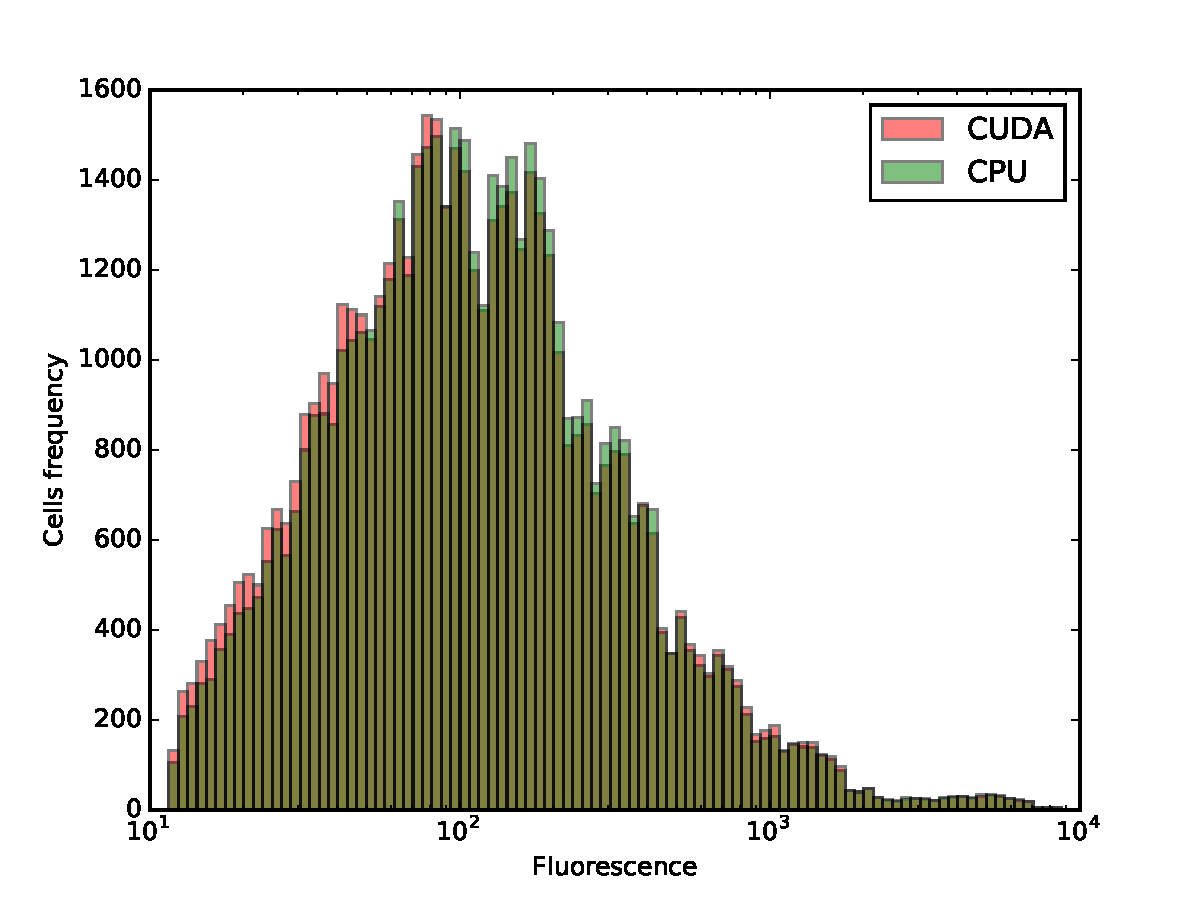
\includegraphics[scale=0.3]{fit_cuda_cpu_comparison}
        \subcaption{Fitting $\varphi_{min}=11.0, \tau_{max}=240$}
    \end{minipage}
    \begin{minipage}[b]{.5\linewidth}
        \centering
        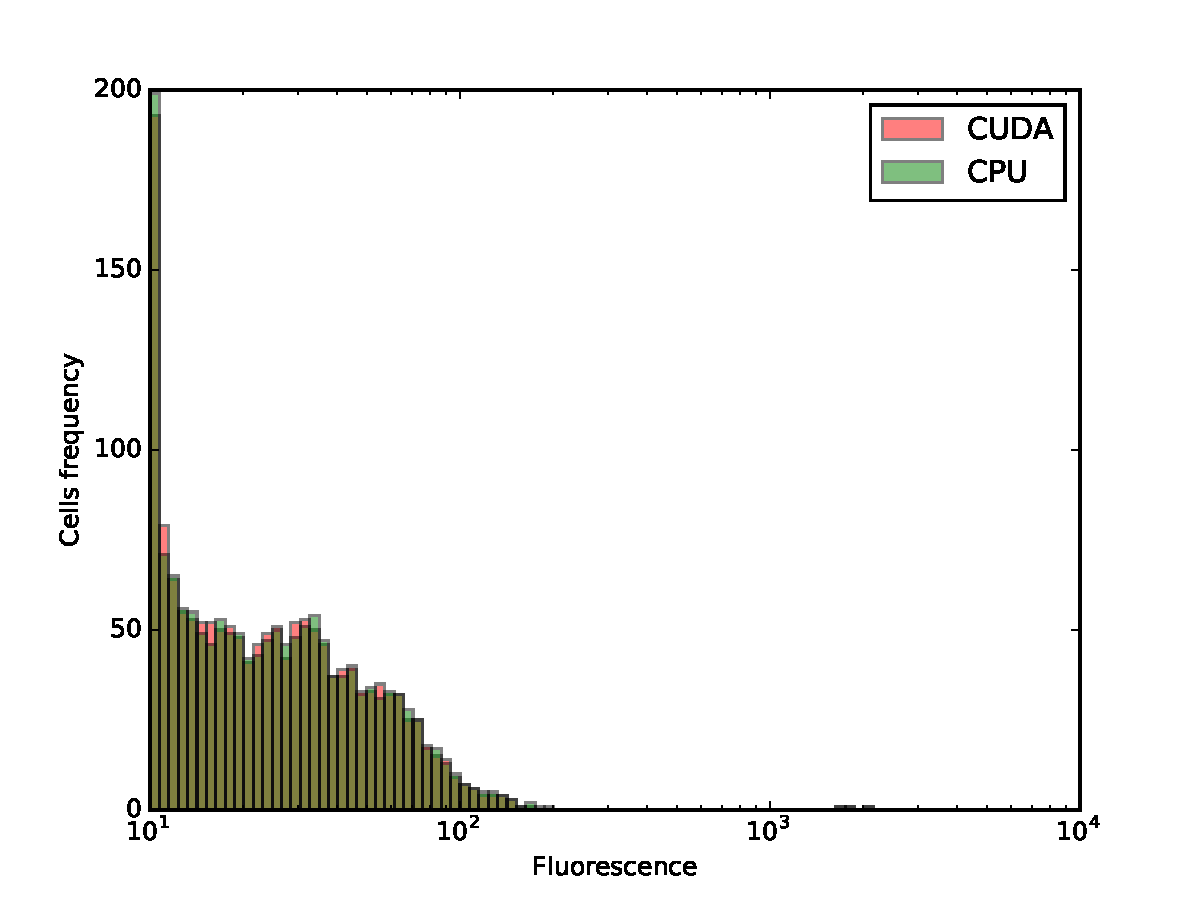
\includegraphics[scale=0.3]{validation_cuda_cpu_comparison}
        \subcaption{Validation $\varphi_{min}=8.7, \tau_{max}=504$}
    \end{minipage}
    \begin{minipage}[b]{.5\linewidth}
        \centering
        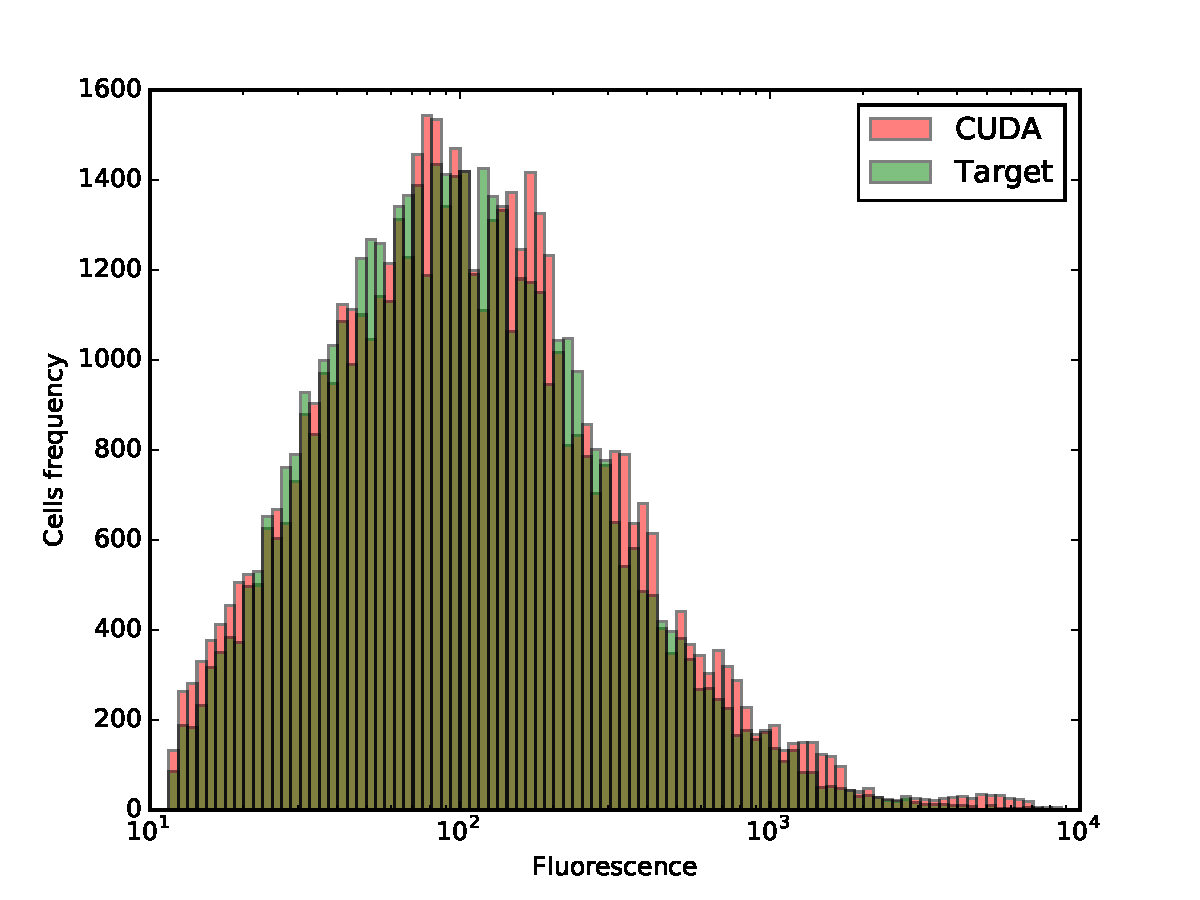
\includegraphics[scale=0.3]{fit_cuda_target_comparison}
        \subcaption{Fitting $\varphi_{min}=11.0, \tau_{max}=240$}
    \end{minipage}
    \begin{minipage}[b]{.5\linewidth}
        \centering
        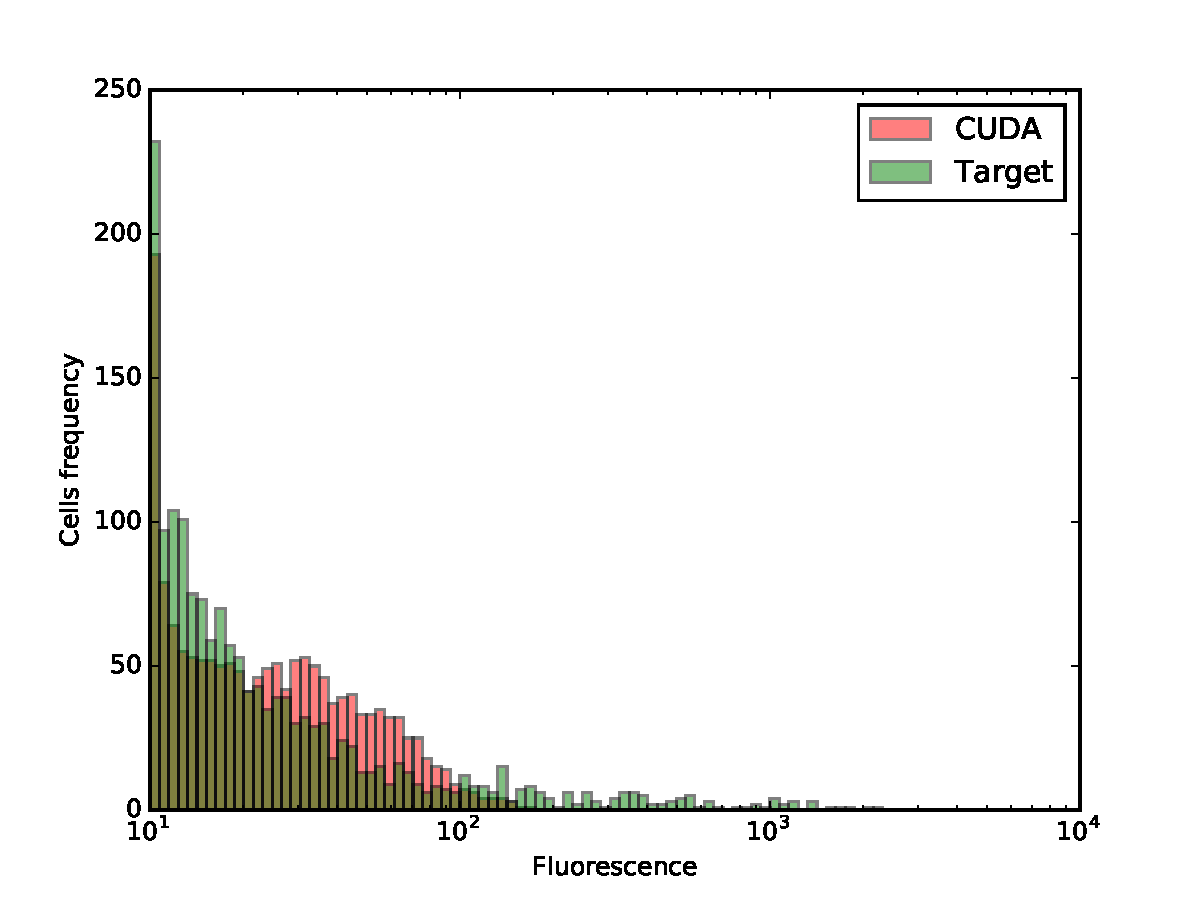
\includegraphics[scale=0.3]{validation_cuda_target_comparison}
        \subcaption{Validation $\varphi_{min}=8.7, \tau_{max}=504$}
    \end{minipage}
    \caption{}
\end{figure}

Come è possibile notare dai grafici in figura, sono presenti aree in cui
i valori di frequenza si discostano tra loro di poche unità. Questa variazione
è dovuta al fatto che la simulazione deve elaborare eventi di tipo stocastico,
dunque il numero di cellule aventi un determinato tipo e il timer di divisione
non saranno mai esattamente uguali per ogni simulazione che si andrà ad
effettuare, e questa situazione è appunto evidenziata dalle aree del grafico
dove è assente l'overlap dei valori. 
